\section{Simulations}

Our experiments apply feedback alignment algorithm to network training on both synthetic and real-world data, where a range of networks with different activation functions and levels of regularization are considered. In particular, we compare the regularized feedback alignment (\cref{algo:fa-reg}) with its non-regularized counterpart (\cref{algo:fa}) on two-layer networks. We also evaluate the regularized feedback alignment algorithm with two-layer classification networks on \texttt{MNIST} dataset.

\paragraph{Feedback alignment on synthetic dataset.}

For two-layer linear networks, the synthetic data for training are drawn from random linear models, where data $x_i$'s are independently generated and have independent standard Gaussian entries. The model parameter $\zeta\in\Rd$ is also independently generated with standard Gaussian entries, and the training label $y_i$ corresponding to $x_i$ is given by $y_i = x_i\transpose \zeta$. In our experiments, each time $n = 50$ data-label pairs $(x_i,y_i)$ are sampled from a random linear model with dimension $d = 150$, which forms one training dataset $(X,y)$ by stacking them as row vectors.

For two-layer non-linear networks, the generation process of training datasets is customized for different networks following the notion of a teacher-student model. If we deem the network to be trained as a student model, its training dataset is generated by a corresponding teacher model that is an independent and randomly initialized network of the same size and architecture. For each network $f$, its training data $x_i$'s are generated as independent Gaussian vectors like in the random linear model, and their corresponding labels are generated as the outputs of a two-layer network $y_i = f'(x_i)$, where $f'$ is an independent replica of $f$ with random Gaussian first- and second-layer weights. More specifically, if $f$ is a network with ReLU activation and hidden layer width $p$, then $f'$ is also a network with ReLU activation and hidden layer width $p$. In our experiments, all the training datasets $(X,y)$ consist of $n = 50$ training samples with dimension $d = 150$ and the training labels generated from an independent replica of the corresponding network.

\begin{figure}[h]
\centering
\begin{subfigure}[b]{.49\textwidth}
  \centering
  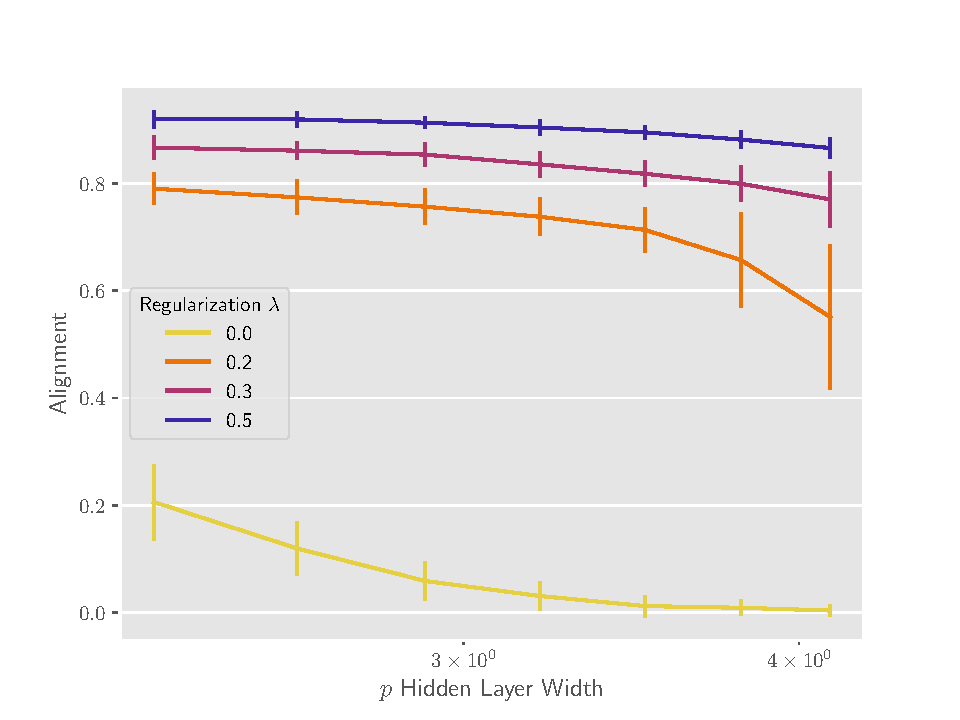
\includegraphics[width=\linewidth]{figures/align_lr_non_autograd_l2_v6.pdf}
  \caption{Feedback alignment and regularized feedback alignment with two-layer linear network on synthetic data.}
  \label{fig:align_lr_non_autograd_l2}
\end{subfigure}\hfill
\begin{subfigure}[b]{.49\textwidth}
  \centering
  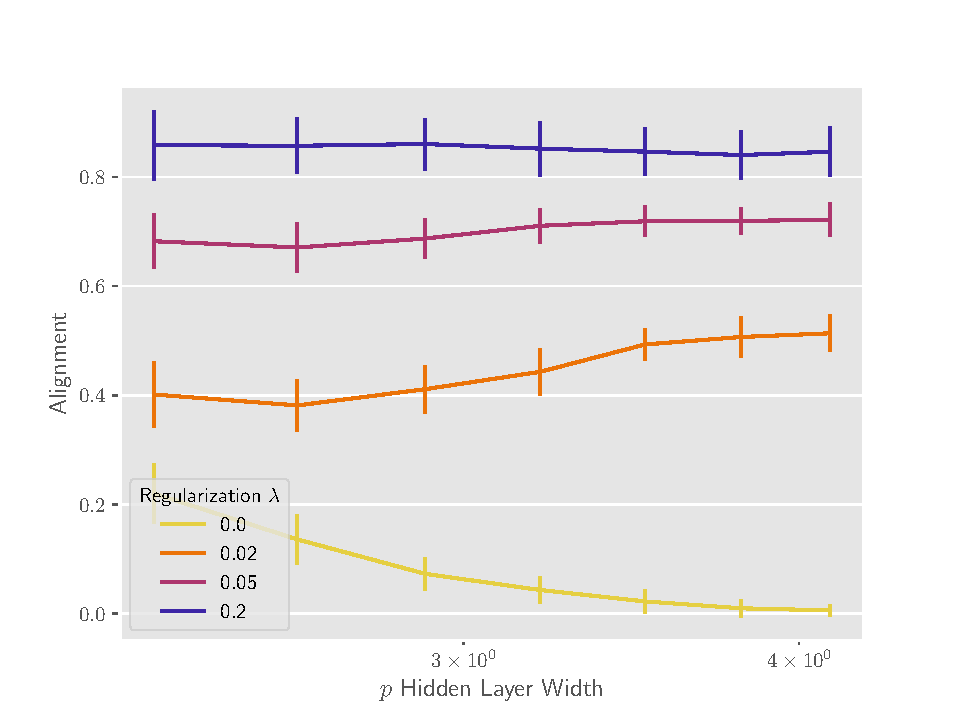
\includegraphics[width=\linewidth]{figures/align_nn_relu_autograd_l2_v6.pdf}
  \caption{Feedback alignment and regularized feedback alignment with two-layer ReLU network on synthetic data.}
  \label{fig:align_nn_relu_autograd_l2}
\end{subfigure}
\medskip
\begin{subfigure}[b]{.49\textwidth}
  \centering
  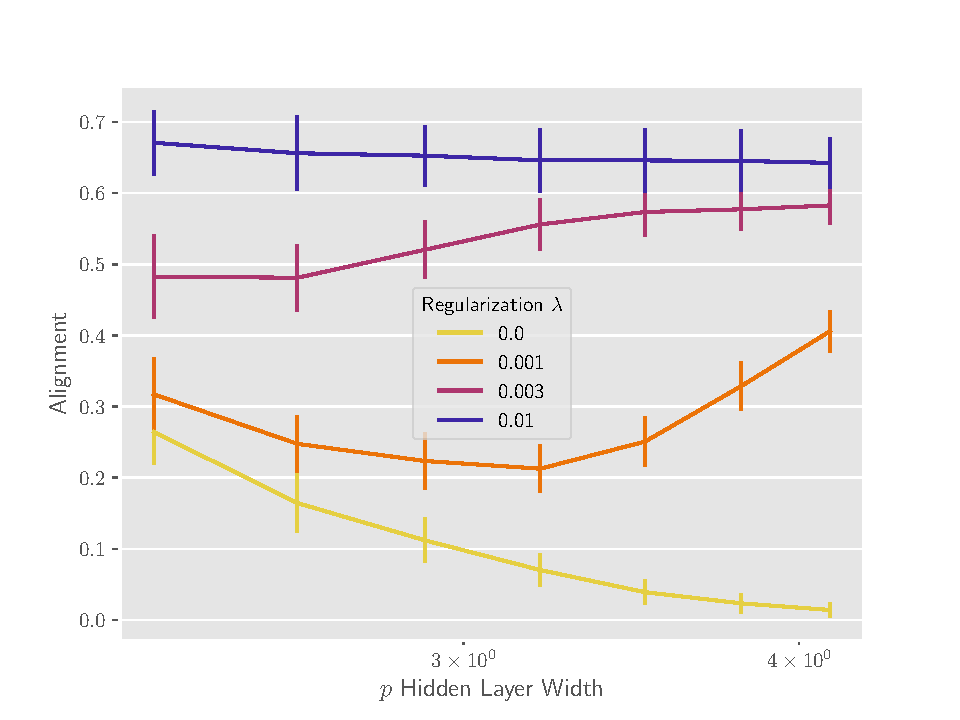
\includegraphics[width=\linewidth]{figures/align_nn_sigmoid_autograd_l2_v6.pdf}
  \caption{Feedback alignment and regularized feedback alignment with two-layer sigmoid network on synthetic data.}
  \label{fig:align_nn_sigmoid_autograd_l2}
\end{subfigure}\hfill
\begin{subfigure}[b]{.49\textwidth}
  \centering
  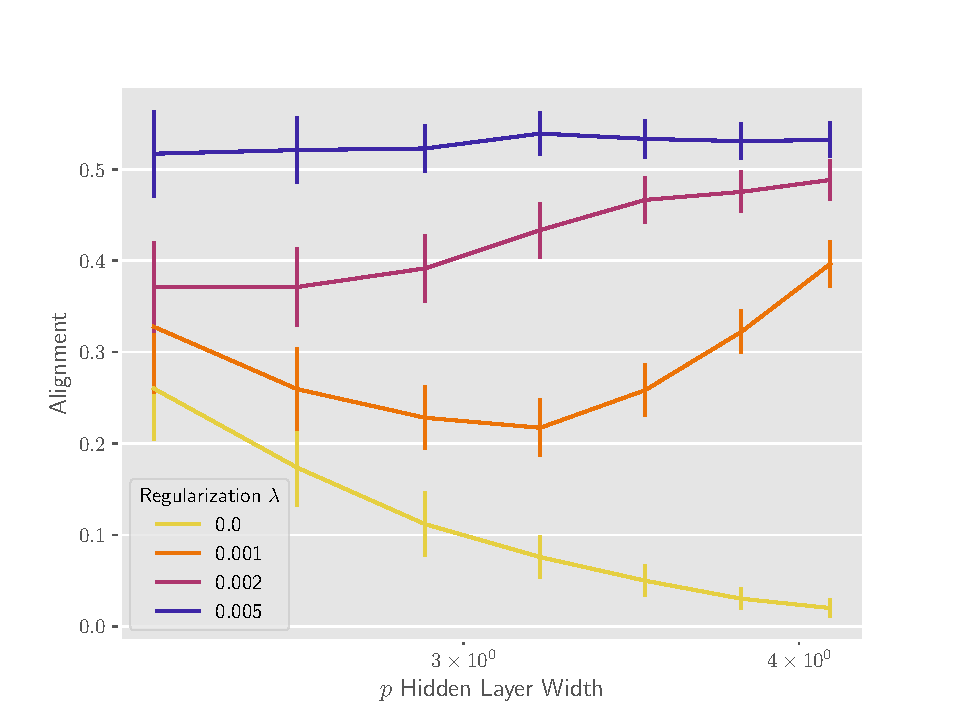
\includegraphics[width=\linewidth]{figures/align_nn_tanh_autograd_l2_v6.pdf}
  \caption{Feedback alignment and regularized feedback alignment with two-layer Tanh network on synthetic data.}
  \label{fig:align_nn_tanh_autograd_l2}
\end{subfigure}
\caption{Comparisons on the alignment for feedback alignment algorithm with different levels of $\ell_2$ regularization. In each figure, the $x$-axis denotes the width $p$ of hidden layer, and it is in logarithmic scale; the $y$-axis represents the level of alignment as the normalized inner product between $\beta_t$ and $b$. The data points are the mean value computed across simulations, and the error bars mark the standard deviation among different runs.}
\label{fig:synthetic-l2}
\end{figure}

In \cref{fig:synthetic-l2} we show numerically how alignment depends on the level of regularization and the hidden layer width $p$ when the (regularized) feedback alignment algorithm is applied to two-layer networks with different hidden layer width $p$ and activation $\psi$. In particular, we obtain \cref{fig:align_lr_non_autograd_l2} from performing feedback alignment on linear networks with linear regression data, and \cref{fig:align_nn_relu_autograd_l2,fig:align_nn_sigmoid_autograd_l2,fig:align_nn_tanh_autograd_l2} are the same numerical benchmarks on non-linear networks with ReLU, sigmoid, and tanh activation function, respectively. For each hidden layer width $p$, we randomly initialize a two-layer network with $p$ hidden neurons and randomly generate a corresponding synthetic dataset for training. Starting from the initialization, we then train the network with feedback alignment algorithm on different levels of regularization and record the alignment between feed-forward weights $\beta$ and backward weights $b$ after the loss converges. This procedure is then repeated $50$ times for each $p$, and the simulation results are summarized in their mean and standard deviation. In all the four figures, \ie,  \cref{fig:align_lr_non_autograd_l2,fig:align_nn_relu_autograd_l2,fig:align_nn_sigmoid_autograd_l2,fig:align_nn_tanh_autograd_l2}, the level of alignment goes to zero when the hidden layer width $p$ is large for feedback alignment algorithm without regularization, while the level of alignment is always kept away from zero for regularized feedback alignment. Further, alignment grows along with the level of regularization $\lambda$ for the same network. Such numerical results strongly support our theoretical statements.

We would like to remark that dropout, a commonly used training technique, as a form of regularization can also help the alignment when used together with feedback alignment algorithm \citep{wager2013dropout}. To the best of our knowledge, there is no satisfying theoretical result available that could explain the underlying mechanism.


\paragraph{Feedback alignment on MNIST dataset.}

The training set of \texttt{MNIST} data consists of $6000$ black-and-white images of handwritten digits with dimension $28$ by $28$, and we flatten each of them into an one-dimensional vector of length $784$. The training data $x_i$'s are obtained after normalizing the vectors by their mean and standard deviation, and the test dataset with $1000$ samples can be similarly processed. We remark that the structure of the two-layer ReLU network we use for classification is slightly different from \eqref{eqn:nonlinear-network}. In particular, the output dimension for classification is $10$ instead of $1$ so that we are able to utilize the cross-entropy loss on the categorical label $y_i$. During training, we take a batch size of $60$ so that $100$ steps are taken in each epoch, and the whole training procedure takes $300$ epochs. 

\cref{fig:mnist} shows the performance of (regularized) feedback alignment under different levels of regularization. The figure on the right-hand side shows the development of test accuracy for the classifier during training, and the regularized feedback alignment converges faster to the maximum accuracy for larger regularization $\lambda$. In the first two figures, we show the development of alignment during training, and we can see that alignment grows much faster with larger regularization.

\begin{figure}[t]
  \centering
  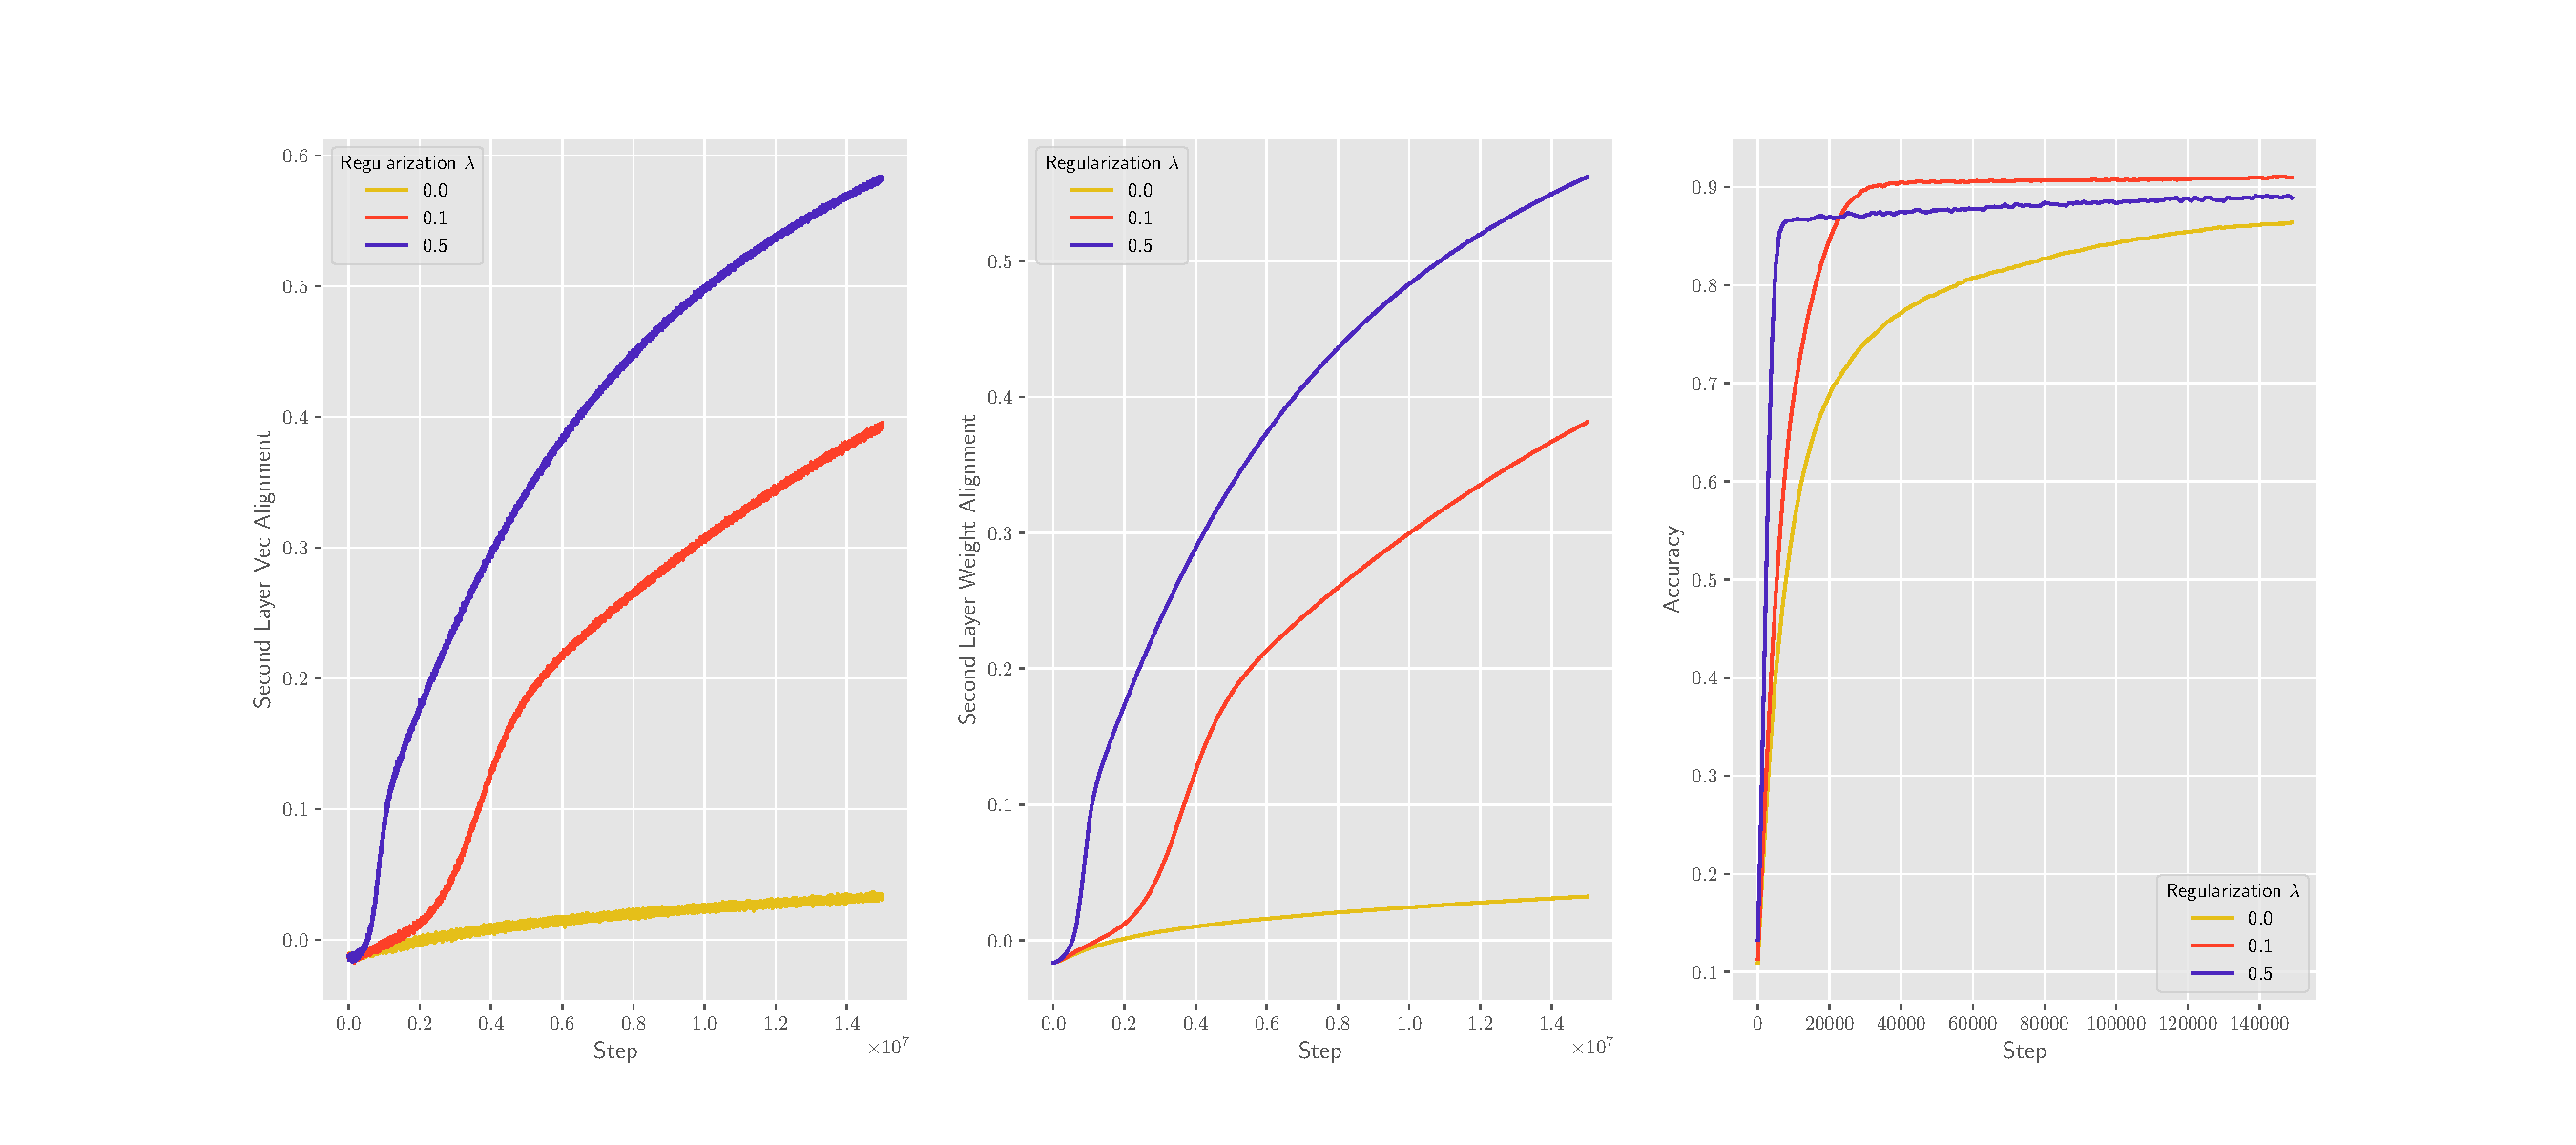
\includegraphics[width=\textwidth]{figures/mnist_2l_v2_horizontal.pdf}
  \caption{\texttt{MNIST} data.}
  \label{fig:mnist}
\end{figure}